\chapter{Time Management}

\section{Roadmap}
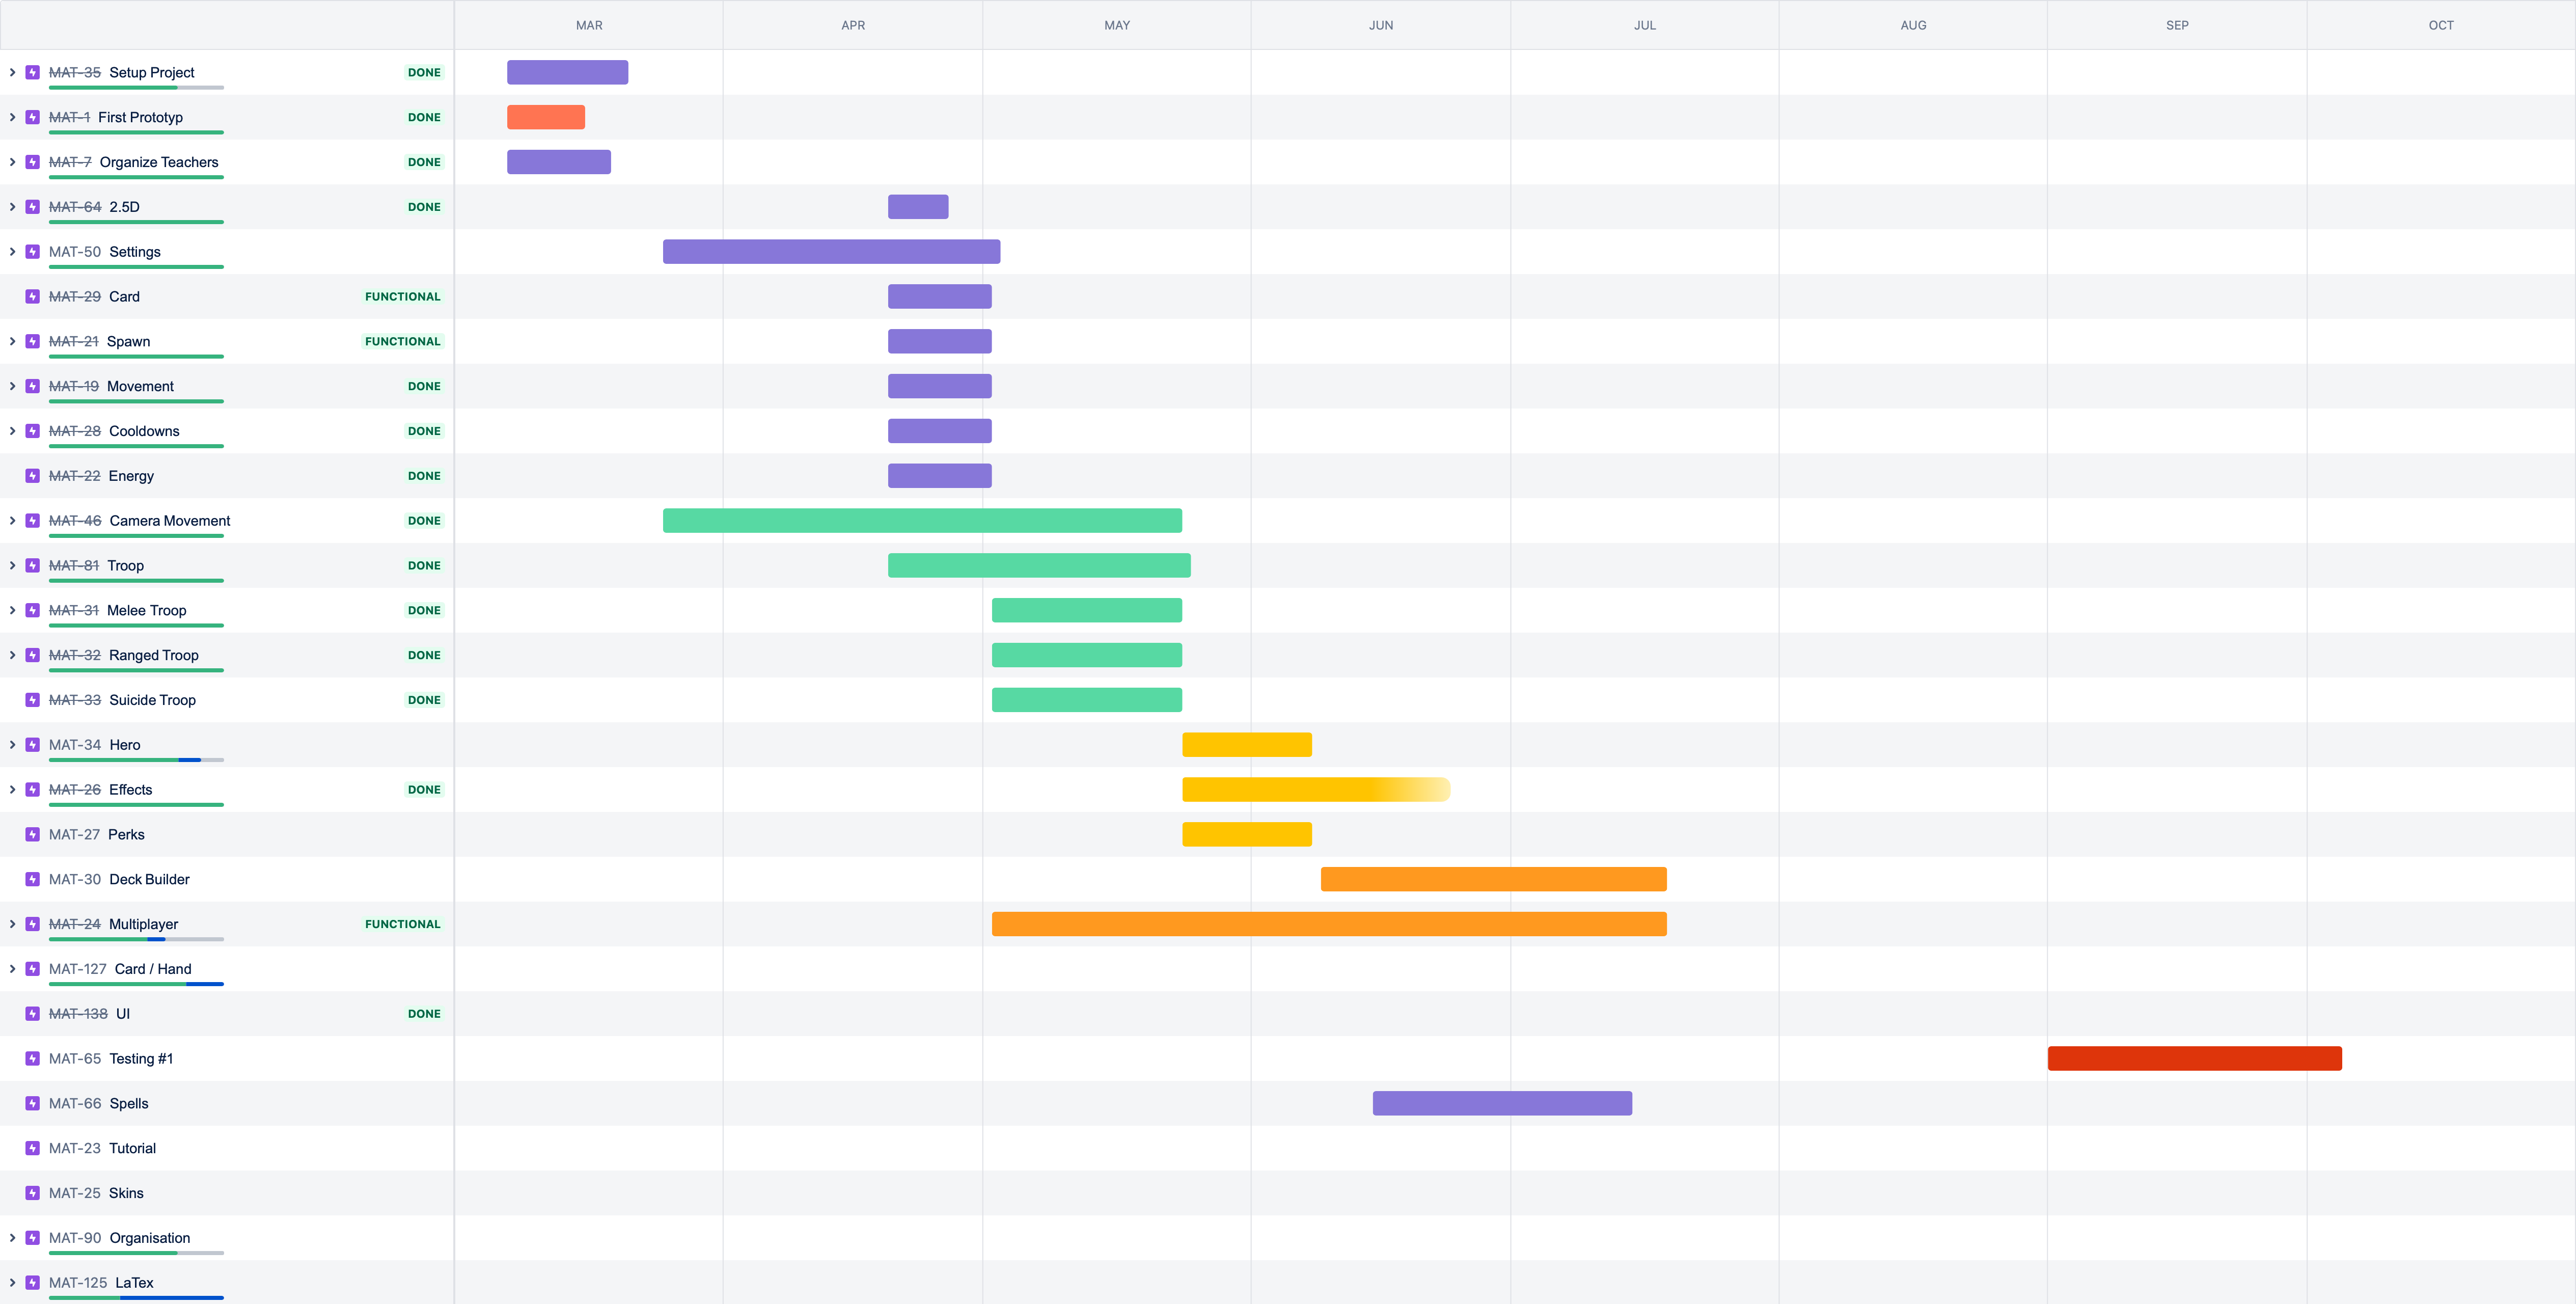
\includegraphics[height=7cm]{resources/Roadmap.png}\\

\section{Time-Tracking}
\includegraphics*[width=15cm]{resources/graph.png}\\

was hat am meisten zeit gebraucht evtl mit kreis graph

HIER NOCH ENDZEITEN IN EXCEL TABELLE SCHREIBEN



%treffen mit hunzi und jezek oder starbucks oder dihei....
%07.03 treffe mit hunzi im inf büro 45m
%08.03 treffe im starbucks vor em theater 3h
%15.03 jezek und hunzi im 1.03 oder so 45m
%20.04 treffe bim marc vor allem roadmap 4h
%04.05 treffe mit hunzi im besprechigszimmer 2.20 2h
%15.6 treffen mit hunzi im 2.20(gruppenzimmer) nach morgenschuel 1h30m
%01.09 treffe mit hunzi nach vormittagsschuel im 12i 1h20m
%23.09 treffe mit hunzi nach 16h 1h 15m
%16.10 starbucks vor bowle 2h

%genauer am anfang festlegen was genau tracken
